%                      Code_Saturne version 1.3
%                      ------------------------
%
%     This file is part of the Code_Saturne Kernel, element of the
%     Code_Saturne CFD tool.
%
%     Copyright (C) 1998-2008 EDF S.A., France
%
%     contact: saturne-support@edf.fr
%
%     The Code_Saturne Kernel is free software; you can redistribute it
%     and/or modify it under the terms of the GNU General Public License
%     as published by the Free Software Foundation; either version 2 of
%     the License, or (at your option) any later version.
%
%     The Code_Saturne Kernel is distributed in the hope that it will be
%     useful, but WITHOUT ANY WARRANTY; without even the implied warranty
%     of MERCHANTABILITY or FITNESS FOR A PARTICULAR PURPOSE.  See the
%     GNU General Public License for more details.
%
%     You should have received a copy of the GNU General Public License
%     along with the Code_Saturne Kernel; if not, write to the
%     Free Software Foundation, Inc.,
%     51 Franklin St, Fifth Floor,
%     Boston, MA  02110-1301  USA
%
%-----------------------------------------------------------------------
%

\programme{matrix}

\vspace{1cm}
%%%%%%%%%%%%%%%%%%%%%%%%%%%%%%%%%%
%%%%%%%%%%%%%%%%%%%%%%%%%%%%%%%%%%
\section{Fonction}
%%%%%%%%%%%%%%%%%%%%%%%%%%%%%%%%%%
%%%%%%%%%%%%%%%%%%%%%%%%%%%%%%%%%%

Le but de ce sous-programme, appel\'e par \fort{codits} et \fort{covofi}, est de construire la
matrice de convection/diffusion, incluant les contributions ad\'equates des termes sources,
intervenant dans le membre de gauche d'\'equations discr\'etis\'ees telles que
celle de la
quantit\'e de mouvement, d'une \'equation de convection diffusion d'un scalaire
ou de mod\`ele de turbulence.\\
Le type d'\'equation consid\'er\'ee est, pour la variable scalaire $a$ :
\begin{equation}\notag
\displaystyle \frac{\partial a}{\partial t} + \dive (\,(\rho \vect{u})\, a) -
\displaystyle \frac{\partial }{\partial x}\left(\beta\,\frac{\partial a}{\partial x}\right) = 0
\end{equation}
La matrice ne s'applique qu'aux termes non reconstruits, les autres \'etant pris en compte au second membre et
trait\'es dans le sous-programme \fort{bilsc2}. La partie
convective, lorsqu'elle existe, est issue du sch\'ema upwind pur, quelque soit
le type de sch\'ema convectif choisi par l'utilisateur. En effet, c'est, \`a
l'heure actuelle, la seule fa\c con d'obtenir un op\'erateur lin\'eaire �
diagonale dominante.\\\\
La matrice est donc associ\'ee \`a $\mathcal{EM_{\it{scal}}}$, op\'erateur
agissant sur un scalaire $a$ (inspir\'e de celui vectoriel $\mathcal{EM}$
d\'efini dans \fort{navsto}) d'expression actuelle, pour tout cellule $\Omega_i$ de
centre $I$  :
\begin{equation}\notag
\begin{array}{lll}
\mathcal{EM_{\it{scal}}}(a,I) &=  f_s^{imp}\ a_I\ \\
&+\sum\limits_{j\in Vois(i)}{F^{\,amont}_{\,ij}((\rho\vect{u})^n,a)}
+\sum\limits_{k\in {\gamma_b(i)}} {F^{\,amont}_{\,{b}_{ik}}((\rho
\vect{u})^n,a)}\\
&-\sum\limits_{j\in Vois(i)}{D^{NRec}_{\,ij}(\beta,a)}
-\sum\limits_{k\in {\gamma_b(i)}} {D^{NRec}_{\,{b}_{ik}}(\beta,a)}\\
\end{array}
\end{equation}
avec~:\\
$\bullet$ $f_s^{imp}$ le coefficient issu du terme instationnaire
$\displaystyle\frac{\rho \ |\Omega_i|}{\Delta t}$, s'il y a lieu, et de
l'implicitation de certains termes sources (contribution d\'ecoulant de la prise
en compte de la
variation $\displaystyle\frac{\partial \rho }{\partial t}$ de
la masse volumique $\rho$ au cours du temps, diagonale du tenseur de pertes de
charges par exemple...): cette initialisation est en fait effectu\'ee en amont
de ce sous-programme, \\
$\bullet$ $F^{\,amont}_{\,ij}$ le flux num\'erique convectif scalaire
d\'ecentr\'e amont calcul\'e \`a la face interne $ij$ de la cellule $\Omega_i$,\\
$\bullet$ $F^{\,amont}_{\,b_{ik}}$ le flux num\'erique convectif scalaire
d\'ecentr\'e amont associ\'e calcul\'e \`a la face de bord $ik$ de la cellule $\Omega_i$
jouxtant le bord du domaine $\Omega$,\\
$\bullet$ $D^{\,NRec}_{\,ij}$ le flux num\'erique diffusif scalaire non
reconstruit associ\'e calcul\'e \`a la face interne $ij$ de la cellule $\Omega_i$,\\
$\bullet$ $D^{\,NRec}_{\,{b}_{ik}}$ le flux num\'erique diffusif scalaire non
reconstruit associ\'e calcul\'e \`a la face de bord $ik$ de la cellule $\Omega_i$ jouxtant le bord du domaine $\Omega$,\\
$\bullet$ $Vois(i)$ repr\'esente toujours l'ensemble des cellules
voisines de ${\Omega_i}$ et $\gamma_b(i)$ l'ensemble des faces de
bord de ${\Omega_i}$.\\
Du fait de la r\'esolution en incr\'ements, $a$ est un incr\'ement et ses
conditions aux limites associ\'ees sont donc de type Dirichlet homog\`ene ou de
type
Neumann homog\`ene.

%%%%%%%%%%%%%%%%%%%%%%%%%%%%%%%%%%
%%%%%%%%%%%%%%%%%%%%%%%%%%%%%%%%%%
\section{Discr\'etisation}
%%%%%%%%%%%%%%%%%%%%%%%%%%%%%%%%%%
%%%%%%%%%%%%%%%%%%%%%%%%%%%%%%%%%%

\begin{figure}[h]
\parbox{8cm}{%
\centerline{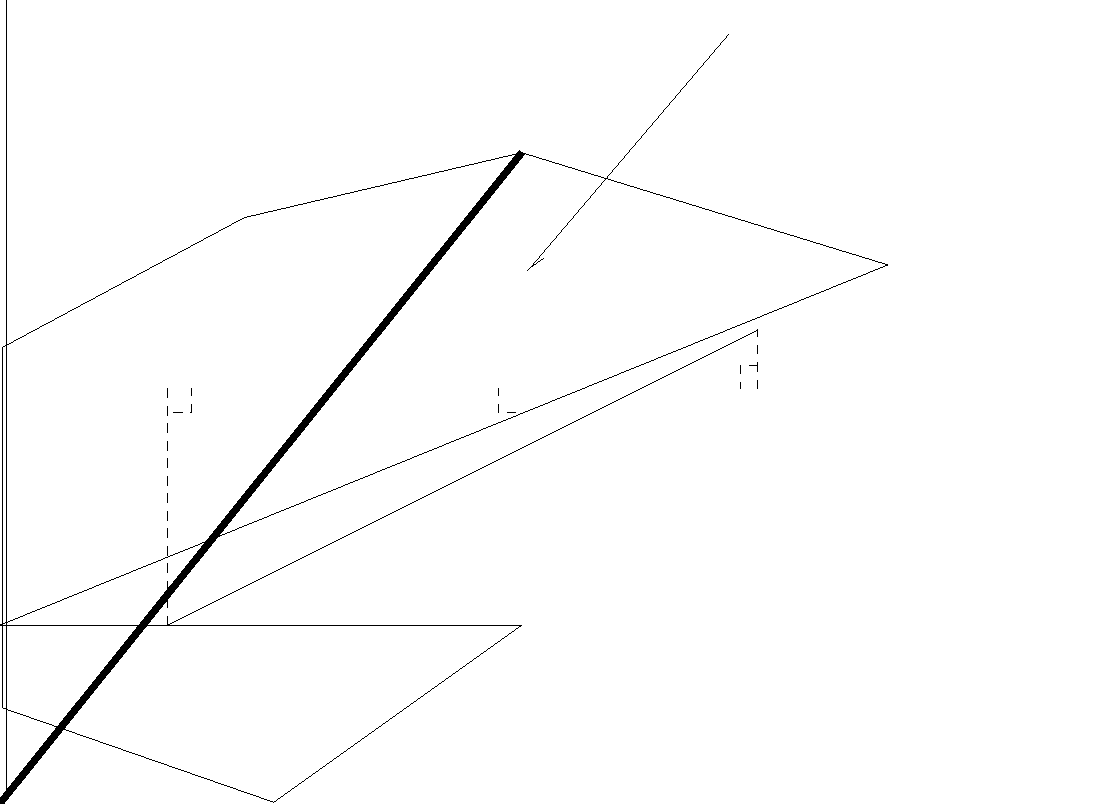
\includegraphics[height=4cm]{\repgraphics/facette}}}
\parbox{8cm}{%
\centerline{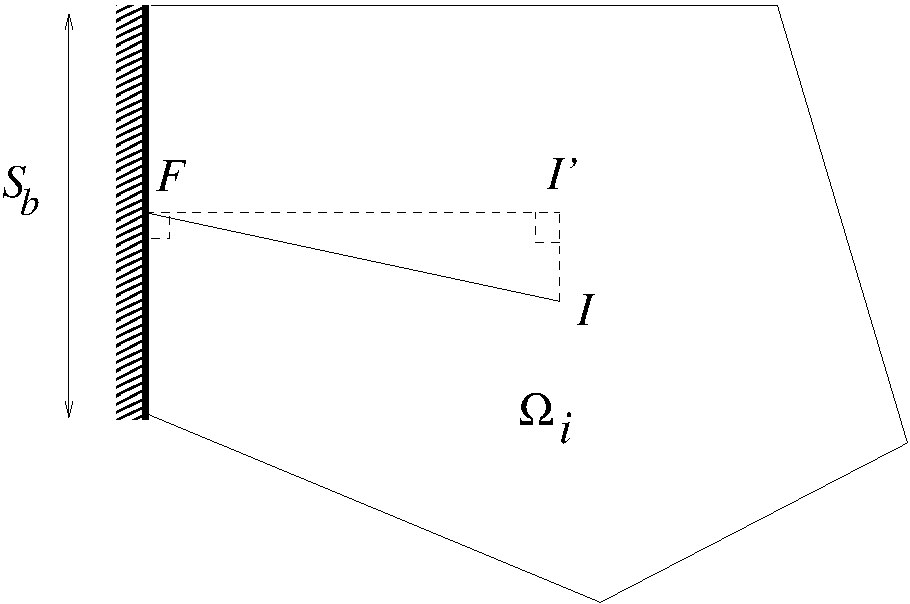
\includegraphics[height=4cm]{\repgraphics/facebord}}}
\caption{\label{Base_Matrix_fig_geom_gradmc}D\'efinition des diff\'erentes entit\'es
g\'eom\'etriques pour les faces internes (gauche) et de bord (droite).}
\end{figure}

L'op\'erateur $\mathcal{EM_{\it{scal}}}$ s'\'ecrit, pour tout $I$ centre de cellule :
\begin{equation}
\begin{array}{lll}
\mathcal{EM_{\it{scal}}}(a,I) &=  f_s^{imp}\ a_I \\
&+\sum\limits_{j\in Vois(i)}\left[{(\rho \vect{u})_{\,ij}^n} \text{.}\, \vect{S}_{\,ij}\right]\ a_{\,f,ij}
+\sum\limits_{k\in {\gamma_b(i)}} \left[{(\rho \vect{u})_{\,{b}_{ik}}^n}
\text{.}\, \vect{S}_{\,{b}_{ik}}\right]\ {a_f}_{\,{b}_{ik}} \\
&-\sum\limits_{j\in Vois(i)} \beta_{\,ij}\displaystyle
\frac{a_{\,J}- a_{\,I}}{\overline{I'J'}} S_{\,ij}
-\sum\limits_{k\in {\gamma_b(i)}} \beta_{\,b_{ik}}\displaystyle
\frac{a_{\,b_{ik}}-a_{\,I}}{\overline{I'F}} S_{\,b_{ik}} \\
\end{array}
\end{equation}
o\`u
$a_{\,f,ij} = a_{\,I} \text{ ou }  a_{\,J}$
selon le signe de $(\rho \vect{u})_{\,ij}^n.\vect{S}_{\,ij}$ (sch�ma
convectif upwind syst�matique),
et avec $\overline{I'J'}$, mesure alg\'ebrique, orient\'ee comme la
normale sortante \`a la face, {\it i.e.} allant de $I$ vers $J$ pour la cellule
$\Omega_i$ de centre $I$. On la
notera ${\overline{I'J'}^{\tiny {\,I}}}$ lorsqu'on aura besoin d'expliciter
clairement l'orientation.\\
${a_f}_{\,{b}_{ik}} = a_I \text{ ou  }
a_{\ {b}_{ik}}$ selon le signe de
${(\rho \vect{u})_{\,{b}_{ik}}^n}\text{.}\, \vect{S}_{\,{b}_{ik}}$ (sch�ma
upwind syst�matique)
et $a_{\ {b}_{ik}}$ valeur au bord est donn\'ee directement par les conditions
aux limites (valeur non reconstruite). $\overline{I'F}$, mesure alg\'ebrique, orient\'ee relativement \`a la
normale sortante \`a la face, {\it i.e.} allant de $I$ vers l'ext\'erieur du domaine.\\
En g\'en\'eral, sauf cas pathologiques, les mesures alg\'ebriques
$\overline{I'J'}$ et $\overline{I'F}$
sont positives et correspondent aux distances $I'J'$ et $I'F$. On se reportera
au paragraphe Points \`a traiter pour plus de d\'etails.\\
Soit ${\tens{EM}}_{\,scal}$ la matrice associ\'ee ; sa taille est {\it a priori} de
$\var{NCEL} * \var{NCEL}$, mais compte-tenu de la nature de la structure de
donn\'ees, seuls deux tableaux \var{DA(NCEL)} contenant les valeurs
diagonales et \var{XA(NFAC,*)} les contributions des termes extra-diagonaux sont n\'ecessaires, avec \var{NCEL} nombre de
cellules du maillage consid\'er\'e et \var{NFAC} nombre de faces internes associ\'e.\\
Du fait des simplifications effectu\'ees sur la matrice (non reconstruction des
termes), les composantes extradiagonales de la ligne $I$ ne sont diff\'erentes de z\'ero que pour
les indices $J$ des cellules voisines de $I$. On peut donc stocker toutes les
contributions non nulles de la matrice dans deux tableaux \var{DA(NCEL)} et \var{XA(NFAC,2)} :\\
$\bullet$ \var{DA(I)} est le coefficient de la colonne $I$ dans la ligne $I$,\\
$\bullet$ si \var{IFAC} est une face qui s\'epare les cellules $\Omega_i$
et $\Omega_j$, orient\'ee de $I$ vers $J$, alors :\\
$\var{XA(IFAC,1)}$ est le coefficient de la colonne $J$ dans la ligne $I$ et
$\var{XA(IFAC,2)}$ est le coefficient de la colonne $I$ dans la ligne $J$.
Lorsque la matrice est sym\'etrique, {\it
i.e.} lorsqu'il n'y a pas de convection (\var{ICONVP} = 0) et que seule la
diffusion est \`a prendre en compte, alors $\var{XA(IFAC,1)} = \var{XA(IFAC,2)}
$ et on r\'eduit \var{XA} \`a $\var{XA(NFAC,1)}$.\\\\
Soit $m_{\,ij}^n$ (\ $m_{\,{b}_{ik}}^n$\ ) la valeur de $(\rho
\vect{u})_{\,ij}^n.\vect{S}_{\,ij}$ (respectivement $(\rho
\vect{u})_{\,{b}_{ik}}^n\text{.}\,\vect{S}_{\,{b}_{ik}}$).\\
Alors~:\\
\hspace*{1cm}{\tiny$\blacksquare$}\ \underline{contribution volumique} : $ f_s^{\,imp}\ a_I $\\\\
\hspace*{1cm}{\tiny$\blacksquare$}\ \underline{contribution d'une face purement interne $ij$} \\
L'expression \\
\begin{equation}\notag
+ \sum\limits_{j\in Vois(i)}{F^{\,amont}_{\,ij}((\rho \vect{u})^n, a)}
- \sum\limits_{j\in Vois(i)}{D^{NRec}_{\,ij}(\,\beta, a)}
\end{equation}
 s'\'ecrit :
\begin{equation}\label{Base_Matrix_eq_face_int}
\begin{array}{ll}
&\ \sum\limits_{j\in Vois(i)}\displaystyle\left({ \left[{(\rho \vect{u})_{\,ij}^n} \text{.}\,
\vect{S}_{\,ij}\right]\ \ a_{\,f,ij} - \beta_{\,ij}\frac{a_J - a_I}{\overline{I'J'}} S_{\,ij}}\right)\\
&=\sum\limits_{j\in Vois(i)}\left[\displaystyle\frac{1}{2}(\  m_{\,ij}^n + |\
m_{\,ij}^n|\ )\,a_I + \displaystyle\frac{1}{2}(\ m_{\,ij}^n - |\
m_{\,ij}^n|)\,a_J\right] - \sum\limits_{j\in Vois(i)}\displaystyle \beta_{\,ij}\frac{a_J - a_I}{\overline{I'J'}} S_{\,ij}
\end{array}
\end{equation}\\
Ici, $\overline{I'J'} = {\overline{I'J'}^{\tiny {\,I}}}$.\\\\
\hspace*{1cm}{\tiny$\blacksquare$}\ \underline{contribution d'une face de bord $ik$} \\
De m\^eme :
\begin{equation}\label{Base_Matrix_eq_face_bord}
\begin{array}{ll}
&\ \sum\limits_{k\in {\gamma_b(i)}} {F^{\,amont}_{\,{b}_{ik}}((\rho \vect{u})^n,a)}
- \sum\limits_{k\in {\gamma_b(i)}} {D^{NRec}_{\,{b}_{ik}}(\beta, a)}\\
&=\sum\limits_{k\in {\gamma_b(i)}}\displaystyle\left(\left[{(\rho
\vect{u})_{\,{b}_{ik}}^n} \text{.}\, \vect{S}_{\,{b}_{ik}}\right]\
{a_f}_{\,{b}_{ik}} - \beta_{\,b_{ik}}
\frac{a_{\,b_{ik}}- a_I}{\overline{I'F}} S_{\,b_{ik}}\right)\\
&=\sum\limits_{k\in {\gamma_b(i)}}\left[\displaystyle\frac{1}{2}(\ m_{\,{b}_{ik}}^n + |\ m_{\,{b}_{ik}}^n|\ )\,a_I +
\displaystyle\frac{1}{2}(\ m_{\,{b}_{ik}}^n -
|m_{\,{b}_{ik}}^n|)\,a_{\,{b}_{ik}}\right] - \sum\limits_{k\in {\gamma_b(i)}}\displaystyle\beta_{\,b_{ik}}
\frac{a_{\,b_{ik}}- a_I}{\overline{I'F}} S_{\,b_{ik}}
\end{array}
\end{equation}
avec~:
\begin{equation}\notag
a_{\,{b}_{ik}} = \var{INC}\,A_{\,b,ik} + B_{\,b,ik}\,a_I =  B_{\,b,ik}\,a_I
\end{equation}
$a$ n'\'etant associ\'ee qu'\`a des conditions aux limites de type Dirichlet
homog\`ene ou de type Neumann homog\`ene.

%%%%%%%%%%%%%%%%%%%%%%%%%%%%%%%%%%
%%%%%%%%%%%%%%%%%%%%%%%%%%%%%%%%%%
\section{Mise en \oe uvre}
%%%%%%%%%%%%%%%%%%%%%%%%%%%%%%%%%%
%%%%%%%%%%%%%%%%%%%%%%%%%%%%%%%%%%
\subsection{\bf Initialisations}
L'indicateur de sym\'etrie \var{ISYM} de la matrice consid\'er\'ee est affect\'e comme suit :\\
\hspace*{1cm}$\bullet$ $\var{ISYM}$ = 1 , si la matrice est sym\'etrique ;
on travaille en diffusion pure , \var{ICONVP} = 0 et \var{IDIFFP} = 1,\\
\hspace*{1cm}$\bullet$ $\var{ISYM}$ = 2 , si la matrice est non sym\'etrique ;
on travaille soit en convection pure (~\var{ICONVP}~=~1, \var{IDIFFP}~=~0~), soit en
convection/diffusion (~\var{ICONVP}~=~1,~\var{IDIFFP}~=~1~).\\
Les termes diagonaux de la matrice sont stock\'es dans le tableau
$\var{DA(NCEL)}$. Ceux extra-diagonaux le sont dans $\var{XA(NFAC,1)}$ si la
matrice est sym\'etrique, dans $\var{XA(NFAC,2)}$ sinon.


Le tableau $\var{DA}$ est initialis\'e \`a z\'ero pour un calcul avec
$ \var{ISTATP} = 0 $ (en fait, ceci ne concerne que les calculs relatifs \`a la
pression). Sinon, on lui affecte la valeur \var{ROVSDT} comprenant la partie instationnaire, la contribution du terme continu en $-\ a\ \dive(\rho \vect{u})^n$
et la partie diagonale des termes sources implicit\'es. Le tableau
$\var{XA(NFAC,*)}$ est initialis\'e \`a z\'ero.\\
\subsection{\bf Calcul des termes extradiagonaux stock\'es dans \var{XA} }
Ils ne se calculent que pour des faces purement internes \var{IFAC}, les faces
de bord ne contribuant qu'\`a la diagonale.
\subsubsection{matrice non sym\'etrique ( pr\'esence de convection ) }
%\hspace*{1cm}{\tiny$\blacksquare$}\ \underline{pour une face purement interne
%$ij\ ( \var{IFAC} )$} \\
Pour chaque face interne \var{IFAC}, les contributions extradiagonales relatives
au terme $a_I$ et \`a son voisin  associ\'e $a_J$ sont calcul\'ees dans
$\var{XA(IFAC,1)}$ et $\var{XA(IFAC,2)}$ respectivement (pour une face orient�e
de I vers J).\\
On a les relations suivantes :\\
\begin{equation}\label{Base_Matrix_eq_extra}
\begin{array}{ll}
\var{XA(IFAC,1)}& = \var{ICONVP}\,*\,\var{FLUI} - \var{IDIFFP}\,*\,\var{VISCF(IFAC)}\\
\var{XA(IFAC,2)}& = \var{ICONVP}\,*\,\var{FLUJ} - \var{IDIFFP}\,*\,\var{VISCF(IFAC)}\\
\end{array}
\end{equation}
avec $\var{FLUMAS(IFAC)}$  correspondant \`a $\ m_{\,ij}^n$, $\var{FLUI}$ \`a $ \displaystyle\frac{1}{2}\,(\ m_{\,ij}^n - |\
m_{\,ij}^n|\ )$, $\var{VISCF(IFAC)} $ \`a $ \ \displaystyle \beta_{\,ij}\frac {
S_{\,ij}}{\overline{I'J'}} $.\\\\
$\var{XA(IFAC,1)}$ repr\'esente le facteur de $a_J$ dans la
derni\`ere expression de (\ref{Base_Matrix_eq_face_int}).\\

$\var{FLUJ}$ correspond \`a $\ -\displaystyle\frac{1}{2}\,(\ m_{\,ij}^n + |\
m_{\,ij}^n|\ )$. En effet, $\var{XA(IFAC,2)}$ est le facteur de $a_I$ dans l'expression \'equivalente de
la derni\`ere ligne de (\ref{Base_Matrix_eq_face_int}), mais \'ecrite en J.\\
Ce qui donne :\\
\begin{equation}\label{Base_Matrix_eq_extra_J}
\sum\limits_{i\in
Vois(j)}\left[\displaystyle\frac{1}{2}(\ m_{\,ji}^n + |\ m_{\,ji}^n|\ )\,a_J +
\displaystyle\frac{1}{2}(\ m_{\,ji}^n - |\ m_{\,ji}^n|)\,a_I\right]
 - \sum\limits_{i\in Vois(j)}\displaystyle \beta_{\,ji}\frac{a_I - a_J}{\overline{J'I'}} S_{\,ji}
\end{equation}\\
Le terme recherch\'e est donc :
$\ \displaystyle\frac{1}{2}(\ m_{\,ji}^n - |\ m_{\,ji}^n|\ )-\displaystyle
\beta_{\,ji}\frac {S_{\,ji}}{\overline{J'I'}}$ .\\
Or :\\ $ m_{\,ji}^n $ = $\ - m_{\,ij}^n $  ($\vect{S}_{\,ji} = -
\vect{S}_{\,ij}$ et $(\rho \vect{u})_{\,ji}^n\  =\ (\rho \vect{u})_{\,ij}^n\
$), avec $\overline{J'I'}$ mesure alg\'ebrique, orient\'ee relativement \`a la
normale sortante \`a la face, {\it i.e.} allant de $J$ vers $I$. On la note
${\overline{J'I'}^{\tiny {\,J}}}$. \\
On a la relation :\\
\begin{equation}\label{Base_Matrix_Eq_mesure_alg}
\overline{J'I'}^{\tiny {\,J}}=\ \overline{I'J'}^{\tiny {\,I}} = (\ \overline{I'J'})
\end{equation}
d'o\`u la deuxi\`eme \'egalit\'e dans (\ref{Base_Matrix_eq_extra}).
\subsubsection{matrice sym\'etrique ( diffusion pure ) }
Pour chaque face interne \var{IFAC}, la contribution extradiagonale relative au
terme $a_I$ est calcul\'ee dans
$\var{XA(IFAC,1)}$ par la  relation suivante :\\
\begin{equation}
\var{XA(IFAC,1)} =  - \var{IDIFFP}\,*\,\var{VISCF(IFAC)}\\
\end{equation}
avec $\var{VISCF(IFAC)} $ \`a $ \ \displaystyle \beta_{\,ij}\frac {
S_{\,ij}}{\overline{I'J'}} $.
\subsection{\bf Calcul des termes diagonaux stock\'es dans \var{DA} }
\subsubsection{matrice non sym\'etrique ( pr\'esence de convection ) }
Pour chaque face interne $ij\ ( \var{IFAC} )$ s\'eparant les cellules $\Omega_i$
de centre $I$ et $\Omega_j$ de centre $J$, $\var{DA(II)}$ est la quantit\'e en facteur de $a_I$ dans la
derni\`ere expression de (\ref{Base_Matrix_eq_face_int}), soit :
\begin{equation}\label{Base_Matrix_eq_diag_II}
\displaystyle\frac{1}{2}(\ m_{\,ij}^n + |\ m_{\,ij}^n|\ )+\displaystyle
\beta_{\,ij}\frac {S_{\,ij}}{\overline{I'J'}}
\end{equation}
De m\^eme, pour \var{DA(JJ)}, on a :
\begin{equation}\label{Base_Matrix_eq_diag_JJ}
\displaystyle\frac{1}{2}(\ - m_{\,ij}^n + |\ m_{\,ij}^n|\ )+\displaystyle
\beta_{\,ji}\frac {S_{\,ij}}{\overline{I'J'}}
\end{equation}
d'apr\`es l'expression de (\ref{Base_Matrix_eq_extra_J}) et l'\'egalit\'e (\ref{Base_Matrix_Eq_mesure_alg}).\\
L'implantation dans \CS associ\'ee est la suivante~:\\
pour toute face \var{IFAC} d'\'el\'ements voisins $\var{II} =
\var{IFACEL(1,IFAC)}$ et $\var{JJ} = \var{IFACEL(2,IFAC)}$,\\
on ajoute \`a
$\var{DA(II)}$ la contribution crois\'ee $-\var{XA(IFAC,2)}$ ({\it cf.}
(\ref{Base_Matrix_eq_diag_II}))  et
\`a
$\var{DA(JJ)}$ la contribution $-\var{XA(IFAC,1)}$ ({\it cf.}
(\ref{Base_Matrix_eq_diag_JJ})).
\subsection{\bf Prise en compte des conditions aux limites}
Elles interviennent juste dans le tableau \var{DA}, compte-tenu de leur
\'ecriture et d\'efinition. Elles se calculent {\it via} la derni\`ere
expression de (\ref{Base_Matrix_eq_face_bord}). Pour chaque face \var{IFAC}, de l'\'el\'ement
de centre $I$, jouxtant le bord, on s'int\'eresse \`a :
\begin{equation}
\begin{array}{ll}
\sum\limits_{k\in {\gamma_b(i)}}\left[\displaystyle\frac{1}{2}(\ m_{\,{b}_{ik}}^n + |\ m_{\,{b}_{ik}}^n|\ )\,a_I +
\displaystyle\frac{1}{2}(\ m_{\,{b}_{ik}}^n -
|m_{\,{b}_{ik}}^n|)\,a_{\,{b}_{ik}}\right] - \sum\limits_{k\in {\gamma_b(i)}}\displaystyle\beta_{\,b_{ik}}
\frac{a_{\,b_{ik}}- a_I}{\overline{I'F}} S_{\,b_{ik}}
\end{array}
\end{equation}
avec~:
\begin{equation}\notag
a_{\,{b}_{ik}} =  B_{\,b,ik}\,a_I\\
\end{equation}
soit :
\begin{equation}
\begin{array}{ll}
\left(\sum\limits_{k\in {\gamma_b(i)}}\left[\displaystyle\frac{1}{2}(\ m_{\,{b}_{ik}}^n + |\ m_{\,{b}_{ik}}^n|\ )\,+
\displaystyle\frac{1}{2}(\ m_{\,{b}_{ik}}^n -
|m_{\,{b}_{ik}}^n|)B_{\,b,ik}\,\right] + \sum\limits_{k\in {\gamma_b(i)}}\displaystyle\beta_{\,b_{ik}}
\frac{1 -\ B_{\,b,ik}}{\overline{I'F}} S_{\,b_{ik}}\right) a_I
\end{array}
\end{equation}
ce qui, pour le terme sur lequel porte la somme, se traduit par :\\
$\var{ICONVP} * (- \var{FLUJ} + \var{FLUI} * \var{COEFBP(IFAC)} + \var{IDIFFP} *
\var{VISCB(IFAC)} * (\ 1 -\ \var{COEFBP(IFAC)})$ \\ avec,
$\ m_{\,{b}_{ik}}^n\ $ repr\'esent\'e par $\ \var{FLUMAB(IFAC)}\ $,
$\ \displaystyle\frac{1}{2}\ (\
m_{\,{b}_{ik}}^n + |\ m_{\,{b}_{ik}}^n|\ )\ $ par $\ \var{-\ FLUJ}\ $,\\
$\ \displaystyle\frac{1}{2}\ (\ m_{\,{b}_{ik}}^n -
|m_{\,{b}_{ik}}^n|)B_{\,b,ik}\ $ par $\ \var{FLUI}\ $,
$B_{\,b,ik}$ par $\var{COEFBP(IFAC)}$, $\beta_{\,b_{ik}}\displaystyle\frac
{S_{\,b_{ik}}}{\overline{I'F}} $ par $\var{VISCB(IFAC)}$.\\
\subsection{\bf D\'ecalage du spectre}
Lorsqu'il n'existe aucune condition \`a la limite de type Dirichlet et que
$\var{ISTATP} = 0 $ (c'est-\`a-dire pour la pression uniquement), on
d\'eplace le spectre de la matrice ${\tens{EM}}_{\,scal}$ de $\var{EPSI}$  ({\it i.e.} on multiplie chaque terme diagonal par $(1 + \var{EPSI})$ ) afin
de la rendre inversible. \var{EPSI} est fix\'e en dur dans \fort{matrix} \`a
 ${10}^{-7}$.
%%%%%%%%%%%%%%%%%%%%%%%%%%%%%%%%%%
%%%%%%%%%%%%%%%%%%%%%%%%%%%%%%%%%%
\section{Points \`a traiter}
%%%%%%%%%%%%%%%%%%%%%%%%%%%%%%%%%%
%%%%%%%%%%%%%%%%%%%%%%%%%%%%%%%%%%
\etape{Initialisation}
Le tableau \var{XA} est initialis\'e \`a z\'ero lorsqu'on veut annuler la
contribution du terme en
$\displaystyle\frac{\rho \ |\Omega_i|}{\Delta t}$, {\it i.e.} $\var{ISTATP} = 0 $ . Ce qui ne permet donc pas la prise en
compte effective des parties diagonales des termes sources \`a impliciter,
d\'ecid\'ee par l'utilisateur. Actuellement, ceci ne sert que pour la variable
pression et reste donc {\it a priori} correct, mais cette d\'emarche est \`a
corriger dans l'absolu.\\\\
\etape{Nettoyage}
La contribution $\var{ICONVP}\ \var{FLUI}$, dans le calcul du terme
\var{XA(IFAC,1)} lorsque la matrice est sym\'etrique est inutile, car
$\var{ICONVP}\ = 0$. \\\\
\etape{Prise en compte du type de sch\'ema de convection dans
${\tens{EM}}_{\,scal}$}
Actuellement, les contributions des  flux convectifs non reconstruits sont
trait\'ees par sch\'ema d\'ecentr\'e amont, quelque soit le sch\'ema choisi par
l'utilisateur. Ceci peut \^etre handicapant. Par exemple, m\^eme sur
maillage orthogonal, on est oblig\'e de faire plusieurs sweeps pour obtenir une
vitesse pr\'edite correcte. Un sch\'ema centr\'e sans test de pente peut
\^etre implant\'e facilement, mais cette \'ecriture pourrait, dans l'\'etat
actuel des connaissances, entra\^\i ner des instabilit\'es
num\'eriques. Il serait souhaitable d'avoir d'autres sch\'emas tout aussi
robustes, mais plus adapt\'es \`a certaines configurations.\\\\
\etape{Maillage localement pathologique}
Il peut arriver, notamment au bord, que les mesures alg\'ebriques,
$\overline{I'J'}$ ou $\overline{I'F}$ soient n\'egatives (en cas de maillages
non convexes par exemple). Ceci peut engendrer des probl\`emes plus ou moins
graves : perte de l'existence et l'unicit\'e de la solution (l'op\'erateur associ\'e n'ayant plus les bonnes propri\'et\'es de r\'egularit\'e
ou de coercivit\'e), d\'egradation de la matrice (perte de la positivit\'e) et donc r\'esolution par solveur lin\'eaire
associ\'e non appropri\'e (gradient conjugu\'e par exemple).\\
Une impression permettant de signaler et de localiser le probl\`eme serait souhaitable.


